\documentclass[12pt,a4paper,oneside]{article}

\usepackage[QX]{polski}

\usepackage[utf8]{inputenc}
\usepackage{latexsym}
\usepackage{tgpagella}
\usepackage{lmodern}
\usepackage{amsmath,amsthm,amsfonts,amssymb,alltt}
\usepackage{epsfig}
\usepackage{pdflscape}
\usepackage{caption}
\usepackage{indentfirst}
\usepackage{float}
%\usepackage{showkeys}
\bibliographystyle{plabbrv}


\usepackage{color}
\usepackage[polish]{babel}
\usepackage{datetime2}
\usepackage[x11names,dvipsnames,table]{xcolor}
\usepackage{hyperref}
\hypersetup{
pdfauthor={Roman Czapla, Olaf Bar},
colorlinks=True,
linkcolor=darkgray,  % color of internal links (change box color with linkbordercolor)
citecolor=BrickRed,  % color of links to bibliography
filecolor=Magenta,   % color of file links
urlcolor=BlueViolet}	%%pdfpagemode=FullScreen}

% diagramy, grafy itp.
\usepackage{tikz}
\usetikzlibrary{positioning}
\usetikzlibrary{arrows}
\usetikzlibrary{arrows.meta}
\usetikzlibrary{chains,fit,shapes,calc}
\tikzset{main node/.style={circle,fill=blue!20,draw,minimum size=1cm,inner sep=0pt}}

% algorytmy
\usepackage[linesnumbered,lined,commentsnumbered]{algorithm2e}
\SetKwFor{ForEach}{for each}{do}{end for}%
\SetKwFor{ForAll}{for all}{do}{end for}%
\newenvironment{myalgorithm}
{\rule{\textwidth}{0.5mm}\\\SetAlCapSty{}\SetAlgoNoEnd\SetAlgoNoLine\begin{algorithm}}{\end{algorithm}\rule{\textwidth}{0.5mm}}


%---------------------
\overfullrule=2mm
\pagestyle{plain}
\textwidth=15cm \textheight=685pt \topmargin=-25pt \linespread{1.3} 
\setlength{\parskip}{0pt}
\setlength\arraycolsep{2pt}
\oddsidemargin = 0.9cm
\evensidemargin =-0.1cm

\captionsetup{width=.95\linewidth, justification=centering}
%---------------------




\newtheorem{tw}{Twierdzenie}[section]
\newtheorem{lem}[tw]{Lemat}
\newtheorem{co}[tw]{Wniosek}
\newtheorem{prop}[tw]{Stwierdzenie}
\theoremstyle{definition}
\newtheorem{ex}{Przykład}
\newtheorem{re}[tw]{Uwaga}
\newtheorem{de}{Definicja}[section]



\newcommand{\bC}{{\mathbb C}}
\newcommand{\bR}{{\mathbb R}}
\newcommand{\bZ}{{\mathbb Z}}
\newcommand{\bQ}{{\mathbb Q}}
\newcommand{\bN}{{\mathbb N}}
\newcommand{\captionT}[1]{\caption{\textsc{\footnotesize{#1}}}}
\renewcommand\figurename{Rys.}

\numberwithin{equation}{section}
\renewcommand{\thefootnote}{\arabic{footnote})}
%\renewcommand{\thefootnote}{\alph{footnote})}



\begin{document}

% --------------------------------------------
% Strona tytułowa
% --------------------------------------------

\thispagestyle{empty}
\begin{titlepage}
\begin{center}\Large
Uniwersytet Komisji Edukacji Narodowej w Krakowie\\
\large
Instytut Bezpieczeństwa i Informatyki\\
\vskip 10pt
\end{center}
\begin{center}
\centering 
\includegraphics[width=1.0\columnwidth]{images/logo.png}
\end{center}

\begin{center}
 {\bf \fontsize{14pt}{14pt}\selectfont PROJEKT INŻYNIERSKI\\ DOKUMENTACJA UŻYTKOWA}
\end{center}
\vskip 5pt
\begin{center}
 {\bf \fontsize{22pt}{22pt}\selectfont RADAR ODCINKOWY}
\end{center}

\begin{center}
 {\fontsize{12pt}{12pt}\selectfont wykonany przez: }
\end{center}
\begin{center}
 {\bf\fontsize{16pt}{16pt}\selectfont Tomasz Górski}\\
 {\fontsize{12pt}{12pt}\selectfont Nr albumu: 151896 \\\&\\}
 {\bf\fontsize{16pt}{16pt}\selectfont Tomasz Joniec}\\
 {\fontsize{12pt}{12pt}\selectfont Nr albumu: 151861\\\&\\}
 {\bf\fontsize{16pt}{16pt}\selectfont Patryk Golonka}\\
 {\fontsize{12pt}{12pt}\selectfont Nr albumu: 145857}
\end{center}
\begin{center}
 {\fontsize{12pt}{12pt}\selectfont pod opieką:}\\
 {\bf\fontsize{12pt}{12pt}\selectfont dr inż. Grzegorz Sokal, mgr Łukasz Przybytek}
\end{center}

%\mbox{}
\vspace*{\fill}
%\vskip 50pt
\begin{center}
\large
Kraków \the\year\\
(ostatnia aktualizacja: \DTMcurrenttime,\;\today)
\end{center}
\end{titlepage}
\setcounter{page}{0} 
\newpage\null\thispagestyle{empty}
%\setcounter{page}{0} 
%\newpage
%\thispagestyle{empty}

\tableofcontents


\newpage

\section{Szczegółowa dokumentacja użytkowa}
\subsection{Opis funkcjonaliści projektowanego systemu}
\begin{enumerate}
  \item Rejestracja w systemie.
        \begin{figure}[H]
          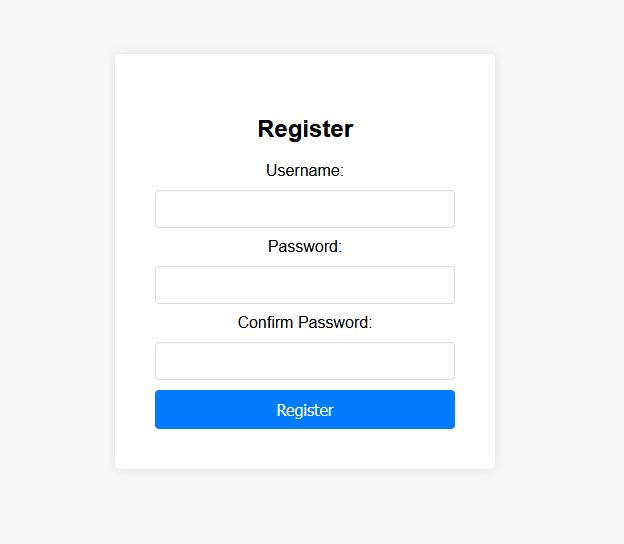
\includegraphics[width=\linewidth]{dokumentacja_uzytkowa/images/register.JPG}
          \label{fig:Rejestracja}
        \end{figure}
        \newpage
  
  \item Logowanie do systemu.
        \begin{figure}[H]
          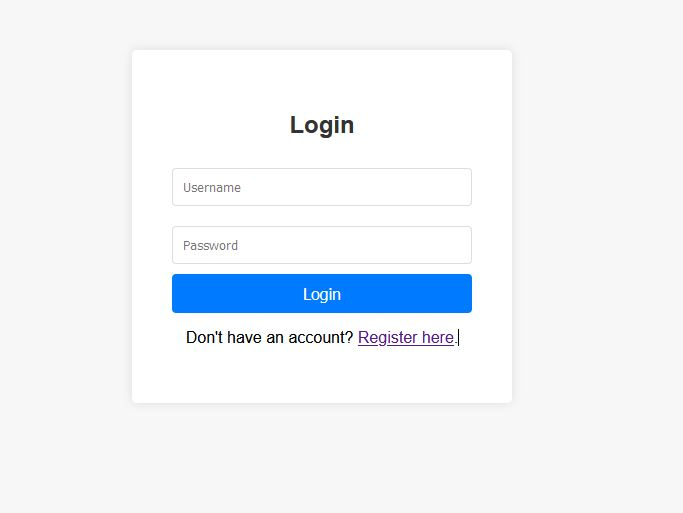
\includegraphics[width=\linewidth]{dokumentacja_uzytkowa/images/login.JPG}
          \label{fig:Logowanie}
        \end{figure}        

  
  \item Prezentacja listy wykrytych zdarzeń przekroczenia prędkości.
        \begin{figure}[H]
          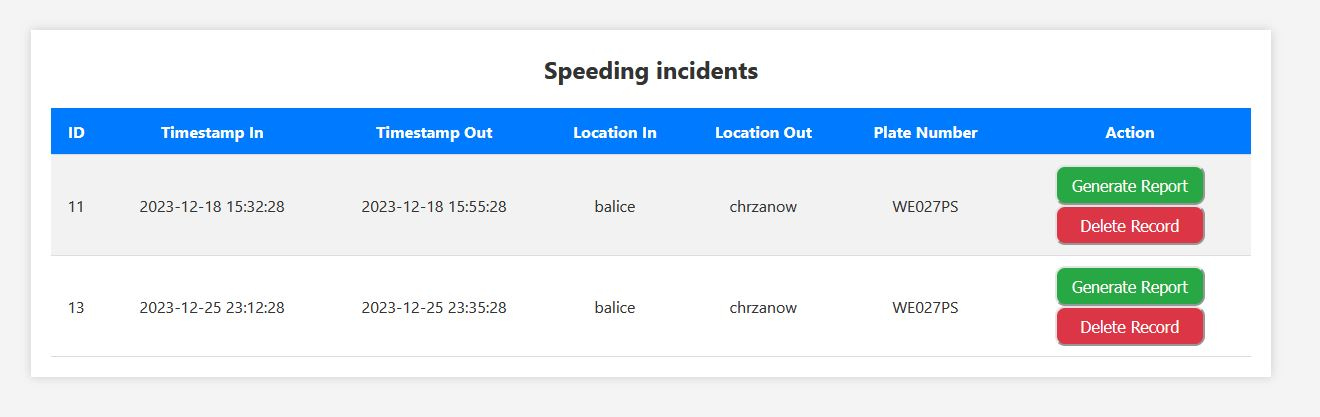
\includegraphics[width=\linewidth]{dokumentacja_uzytkowa/images/incidents.JPG}
          \label{fig:Prezentacja}
        \end{figure}
        \newpage
  
  \item Generowanie raportu ze zdarzenia za pomocą zielonego przycisku "Generate Report". 
        \begin{figure}[H]
          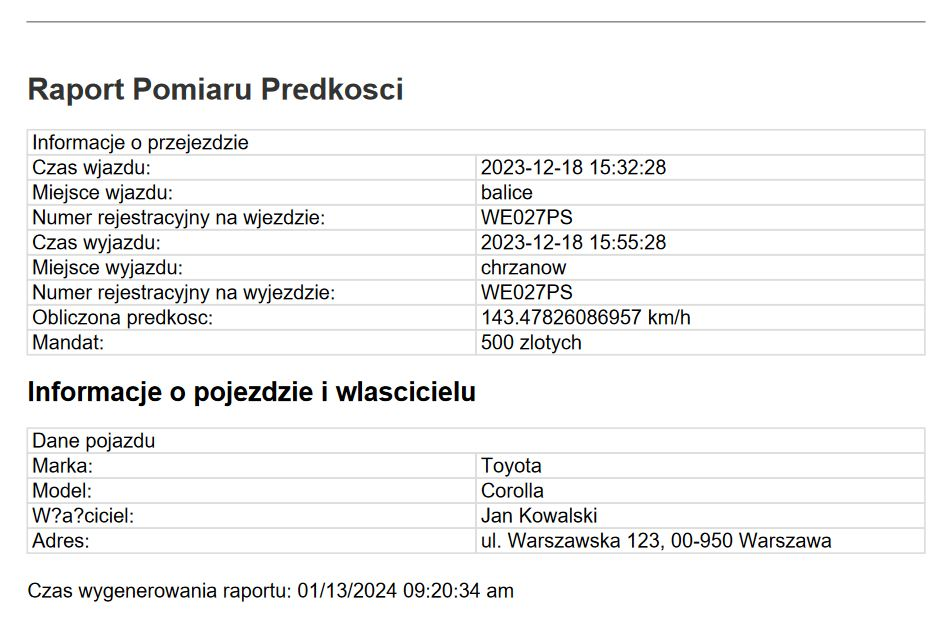
\includegraphics[width=\linewidth]{dokumentacja_uzytkowa/images/report.JPG}
          \label{fig:Generowanie}
        \end{figure}  
  \item Usunięcie rekordu z listy za pomocą czerwonego przycisku "Delete Record". 
        \begin{figure}[H]
          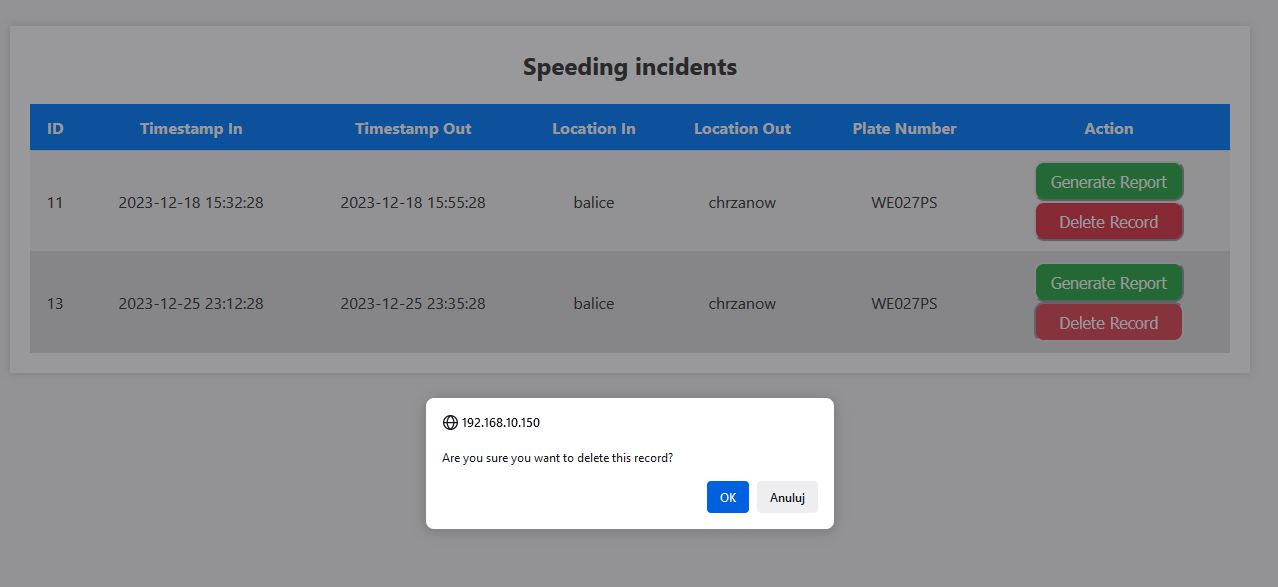
\includegraphics[width=\linewidth]{dokumentacja_uzytkowa/images/delete_1.JPG}
          \label{fig:Usunięcie}
        \end{figure}
        \newpage

  \item Wylogowanie z systemu za poomocą 'Logout' w prawym górnym rogu.
        \begin{figure}[H]
          \centering
          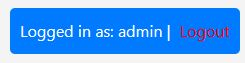
\includegraphics[width=4cm]{dokumentacja_uzytkowa/images/logout.JPG}
          \label{fig:Wylogowanie}
        \end{figure}  
\end{enumerate}








\subsection{Przykładowe działanie systemu}
Aby zaprezentować działanie systemu należy założyć hipotetyczne zdarzenia przekroczenia prędkości:
\begin{enumerate}
  \item Pojazd Toyota Corolla o nr rejestryjnych WE027PS porusza się autostradą.
  \item Samochód przejeżdza przez punkt Balice. Pojazd zostaje rozpoznany przez oprogramowanie kamery, zdjęcie z timepstampem '2023-12-18 15:32:28' zostaje przesłane z kamery IP na serwer FTP natychmiastowo. 
  \item Zgodnie z zaproponowanym ustawieniem crontab o 15:33 zostanie utworzony plik graficzny przedstawiający wyciętą rejestracje, o 15:37 numer rejestracyjny zostanie rozpoznany i informacje o przejeździe zostaną wysłane do bazy danych. 
  \item Następnie pojazd przejeżdza przez punkt Chrzanów. Pojazd zostaje rozpoznany przez oprogramowanie kamery, zdjęcie z timepstampem '2023-12-18 15:55:28' zostaje przesłane z kamery IP na serwer FTP natychmiastowo. 
  \item O 15:57 zostanie utworzony plik graficzny przedstawiający wyciętą rejestracje, o 16:02 numer rejestracyjny zostanie rozpoznany i informacje o przejeździe zostaną wysłane do bazy danych, zostanie zaktualizowany przejazd rozpoczęty o 15:32:28 ze względu na przekroczenie prędkości.
  \item Gdy dane o przejezdzie zostaną w pełni wprowadzone do bazy i zostanie wykryty incydent przekroczenia prędkości to w interfejsie pojawi się odpowiedni wpis. 
        \begin{figure}[H]
          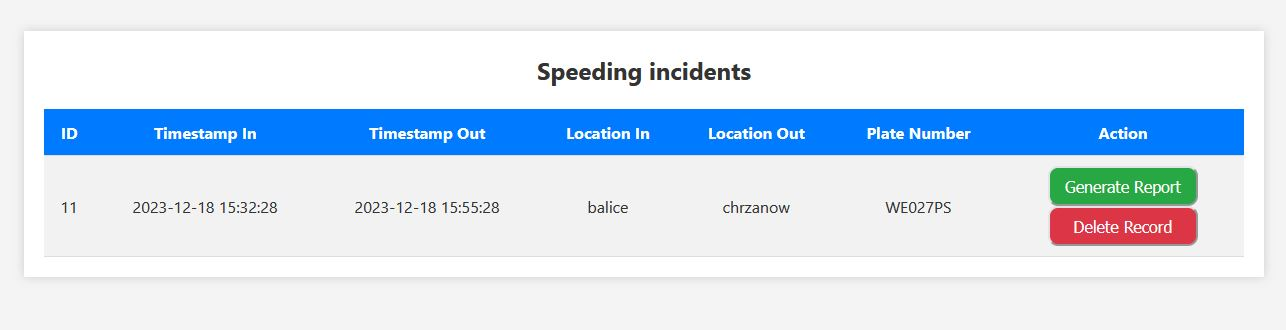
\includegraphics[width=\linewidth]{dokumentacja_uzytkowa/images/delete_2.JPG}
          \label{fig:Generowanie}
        \end{figure}    
  \item Osoba obsługująca system może wygenerować raport ze zdarzenia, załączyć go do mandatu oraz usunąć incydent z listy. 
        \begin{figure}[H]
          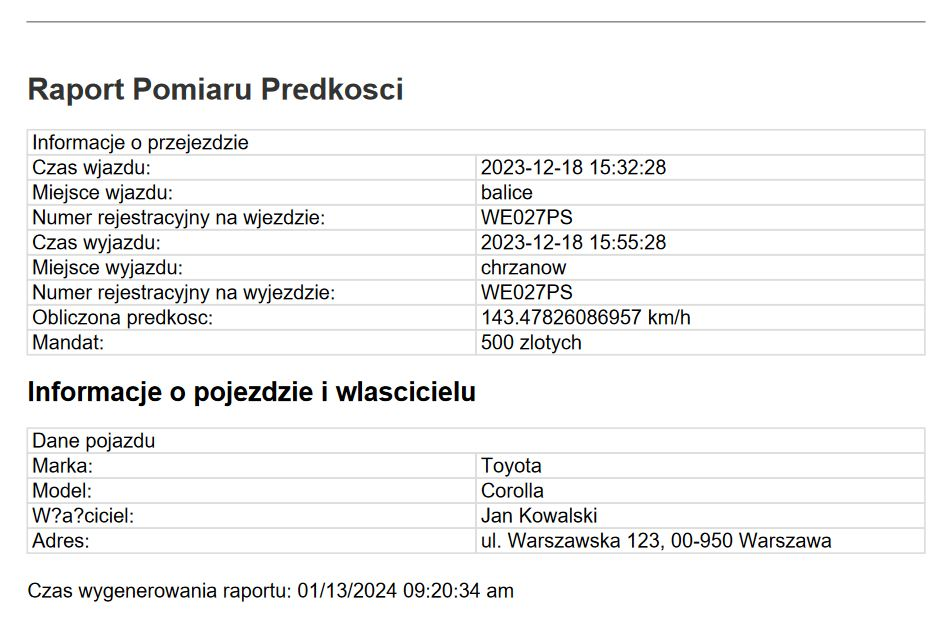
\includegraphics[width=\linewidth]{dokumentacja_uzytkowa/images/report.JPG}
          \label{fig:Generowanie}
        \end{figure}           
\end{enumerate}






% --------------------------------------------------------------------
%%%%%%% odkomentować gdy bibliografia ma być wewnątrz dokumentu
% --------------------------------------------------------------------
%\begin{thebibliography}{11}
%
%\addcontentsline{toc}{section}{Literatura}
%
%\bibitem{ZAN}
%C. Zannoni and P. Pasini, 
%\emph{Advances in the Computer Simulatons of Liquid Crystals}, Kluwer Academic Publishers, 2000.
%
%\end{thebibliography}

\end{document}

